\documentclass{ctexart}
\usepackage{graphicx}
\usepackage{geometry}
\usepackage{amsmath}
\usepackage{amssymb}
\usepackage{mathrsfs}
\usepackage{color}
\usepackage[colorlinks,linkcolor = black]{hyperref}
\usepackage{listings}
\geometry{left = 3cm,right = 3cm,top = 2.5cm, right = 2.5cm}

\definecolor{mygreen}{rgb}{0,0.6,0}
\definecolor{mygray}{rgb}{0.5,0.5,0.5}
\definecolor{mymauve}{rgb}{0.58,0,0.82}
\lstset{ %
	backgroundcolor=\color{white},   % choose the background color
	basicstyle=\ttfamily,        % size of fonts used for the code
	columns=fullflexible,
	breaklines=true,                 % automatic line breaking only at whitespace
	captionpos=b,                    % sets the caption-position to bottom
	tabsize=4,
	commentstyle=\color{mygreen},    % comment style
	escapeinside={\%*}{*)},          % if you want to add LaTeX within your code
	keywordstyle=\color{blue},       % keyword style
	stringstyle=\color{mymauve}\ttfamily,     % string literal style
	frame=single,
	% rulesepcolor=\color{red!20!green!20!blue!20},
	% identifierstyle=\color{red},
	% language=c++,
}

\begin{document}
		\title{CS229 Machine Learning Problem Set 2}
		\author{Wang Minhu}
		\date{12, Sep, 2017}
		\maketitle
		\clearpage
\section{Constructing Kernels}
为以下的讨论约定部分记号, 对任意有限长序列$\{x^{(1)} \cdots x^{(m)}\}$和核函数$K$, 定义$\mathcal{K} \in {\mathbb{R}}^{m \times m}$为${\mathcal{K}}_{ij} = K(x^{(i)}, x^{(j)})$.
向量$\forall v \in R^m$, 有
\begin{equation*}
	v^T \mathcal{K} v \ge 0
\end{equation*}
\paragraph{a}
	对$K(x,z) = K_1(x,z) + K_2(x,z)$
\begin{equation*}
	v^T \mathcal{K} v = v^T (\mathcal{K}_1 + \mathcal{K}_2) v = v^T (\mathcal{K}_1 ) v +  v^T (\mathcal{K}_2) v \ge 0
\end{equation*}

	$K(x,z)$可以作为向量机的核函数.
	
\paragraph{b}
	对$K(x,z) = K_1(x,z) - K_2(x,z)$, $K(x,z)$不必然是核函数.
	
	举一反例, 不妨设$K_1$是核函数, $K_2 = 2K_1(x,z)$.

\begin{equation*}
	v^T \mathcal{K}_2 v = 2	v^T \mathcal{K}_1 v \ge 0
\end{equation*}	

	因此$K_2$是核函数.
	
\begin{equation*}
v^T \mathcal{K} v = v^T (\mathcal{K}_1 - \mathcal{K}_2) v = v^T (\mathcal{K}_1 ) v -  v^T (\mathcal{K}_2) v = - v^T (\mathcal{K}_1) v \le 0
\end{equation*}	
	
	因此$K(x,z)$不是核函数.
	
\paragraph{c}

\begin{equation*}
v^T \mathcal{K} v = v^T a(\mathcal{K}_1) v = a(v^T (\mathcal{K}_1 ) v) \ge 0
\end{equation*}		
	
	$K(x,z)$是核函数
	
\paragraph{d}

\begin{equation*}
v^T \mathcal{K} v = v^T (-a)(\mathcal{K}_1) v = -a(v^T (\mathcal{K}_1 ) v) \le 0
\end{equation*}		

	$K(x,z)$不是核函数	

\paragraph{e}

半正定矩阵可以拆分为矩阵的乘积

\begin{align*}
	\mathcal{K} &= U^T U  \\
	\mathcal{K}_{ij} &= \sum_{k} U_{ki}U_{kj} \\
\end{align*}

则

\begin{align*}
	v^T \mathcal{K} v &= \sum_{ij} v_i \mathcal{K}_{1ij} \mathcal{K}_{2ij} v_j = \sum_{ijk} v_i U_{ki}U_{kj}\mathcal{K}_{2ij} v_j = \sum_{k} \sum_{ij} \mathcal{K}_{2ij} v_i U_{ki}U_{kj} v_j \\
		&= \sum_{k} \sum_{ij} \mathcal{K}_{2ij} (U_{ki} v_i) (U_{kj} v_j) \ge 0 \\
\end{align*}

$K$是核函数

\paragraph{f}

\begin{align*}
v^T \mathcal{K} v &= \sum_{ij} v_i \mathcal{K}_{ij}  v_j = \sum_{ij} v_i f(x^{i})f(x^{j})  v_j
 \\ &= [v_1 f(x^1) \cdots v_n f(x^n)] \begin{bmatrix}
  1 & \cdots & 1 \\
  1 & \cdots & 1 \\
  \cdots & \cdots & \cdots \\
  1 & \cdots & 1 \\
 \end{bmatrix} \begin{bmatrix}
  v_1 f(x^1) \\ \cdots \\ v_n f(x^n)
 \end{bmatrix} \\ &= (\sum_i v_i f(x^i))^2 \ge 0
\end{align*}

$K$是核函数.

\paragraph{g}

对任意$d$阶向量序列, $\{x^{(1)}, \cdots ,x^{(2)}\}$, 满足$K_{ij} = K_3(x^{(i)}, x^{(j)})$的矩阵$K$是正定的. 

对于任意$n$阶向量序列, $\{x^{(1)}, \cdots ,x^{(2)}\}$, $\{ \phi(x^{(1)}), \cdots ,\phi(x^{(2)}) \}$是d阶向量序列, 满足$K_{ij} = K(x^{(i)}, x^{(j)}) = K_3(\phi(x^{(i)}), \phi(x^{(j)})$的矩阵$K$也是正定的.

$K$是核函数.

\paragraph{h}

\begin{align*}
v^T \mathcal{K} v &= \sum_{ij} v_i p(\mathcal{K}_{1_ij})  v_j \\
				&= \sum_{ij} v_i (a_n(\mathcal{K}_{1_ij})^n + a_{n-1}(\mathcal{K}_{1_ij})^{n - 1} + \cdots + a_0)  v_j \\
				&= a_n \sum_{ij} v_i (\mathcal{K}_{1_ij})^n v_j + a_{n-1} \sum_{ij} v_i(\mathcal{K}_{1_ij})^{n - 1} v_j \cdots + \sum_{ij} v_i v_j
\end{align*}

已知$K(x,z) = K_1(x,z)K_2(x,z)$是核函数, 很容易证明$(K_1(x,z))^n$是核函数, 由此$\sum_{ij} v_i (\mathcal{K}_{1_ij})^n v_j \ge 0$. 已知$a_i >0 , 0 \le x \le n$.

\begin{align*}
v^T \mathcal{K} v &= a_n \sum_{ij} v_i (\mathcal{K}_{1_ij})^n v_j + a_{n-1} \sum_{ij} v_i(\mathcal{K}_{1_ij})^{n - 1} v_j \cdots + (\sum_{ij} v_i)^2 \ge 0
\end{align*}

\section{Kernelizing the Perceptron}

注意, 由$\theta$的更新公式

\begin{equation}
\theta^{(i+1)} = \theta^{(i)} + \alpha 1\{\theta^{(i)^T} \phi(x^{(i+1)}) y^{(i+1)} < 0\}  y^{(i+1)}\phi(x^{(i+1)})
\end{equation}

$\theta^{(i)}$可以写成$\phi(x^{(0)}) \cdots \phi(x^{(i)})$的线性组合, 即

\begin{equation}
	\theta^{(i)} = a_0 \phi(x^{(0)}) + \cdots + a_i \phi(x^{(i)})
\end{equation}

由于样本长度是有限的, $i$是一个有限常数. 同时可以使用核函数直接计算$\theta^T x$

\begin{align*}
\theta^{(i)^T}\phi(x^{(i+1)}) &= a_0 \phi(x^{(0)})^T\phi(x) + \cdots + a_i \phi(x^{(i)})^T\phi(x) \\
	&= a_0 K(x^{(0)}, x^{(i+1)}) + \cdots + a_i K(x^{(i)}, x^{(i+1)}) 
\end{align*}

因此$\theta$可以用一个有限长序列$[a_0, a_1, a_2, \cdots]$表示, $\theta_0$可以使用空序列$[ ]$表示.

更新时使用核函数计算$(\theta^{(i)})^T\phi(x^{(i+1)})$, 而后以 $ \alpha 1\{\theta^{(i)^T} \phi(x^{(i+1)}) y^{(i+1)} < 0\}  y^{(i+1)}$ 增长序列.

\section{Spam Classification}

\subsection{}
朴素贝叶斯训练过程代码如下
\begin{lstlisting}[language = MATLAB]
% split the training data set into two parts: Spam and Not Spam.
Spam = trainMatrix(trainCategory == 1,:);
NoSpam = trainMatrix(trainCategory == 0,:);

SpamProb = size(Spam,1) / numTrainDocs;
NoSpamProb = size(NoSpam,1) / numTrainDocs;

% use logarithms to avoid the problem of underflow
SpamWordProb = log((sum(Spam) + 1)/(sum(sum(Spam)) + numTokens)); 
NoSpamWordProb = log((sum(NoSpam) + 1)/(sum(sum(NoSpam)) + numTokens)); 
\end{lstlisting}

误差计算:
\begin{lstlisting}[language = MATLAB]
TestSpamProb = testMatrix * SpamWordProb' + SpamProb;
TestNoSpamProb = testMatrix * NoSpamWordProb' + NoSpamProb;
% if log(SpamProb) > log(NoSpamProb), The email is regarded as SPAM
output = TestSpamProb > TestNoSpamProb;
\end{lstlisting}

\subsection{}
5个效果最好的字段如下[language = MATLAB]
\begin{lstlisting}
[V I] = sort(IndicativeVector, 'descend');
TokenList = split(tokenlist);
ind = I(1:5);
table(ind', V(1:5)', TokenList(ind'), 'VariableName',{'index';'log_p';'token'})
\end{lstlisting}

\begin{verbatim}
index    log_p        token    
_____    ______    ____________

616     6.5993    'httpaddr'  
1210    6.5993    'spam'      
1357    4.9938    'unsubscrib'
394     4.8519    'ebai'      
353     4.6524    'diploma'  
\end{verbatim}

\subsection{}

使用不同大小的训练集训练该分类器, 得到其错误率.
\begin{table}[ht]
	\centering
	\begin{tabular}{|c|c|}
		\hline
		Training data size & test error rate \\
		\hline
		50 & $3.87\%$\\
		100 & $2.62\%$\\
		200 & $2.62\%$\\
		400 & $1.87\%$\\
		800 & $1.75\%$\\
		1400 & $1.63\%$\\
		\hline
	\end{tabular}
	\caption{朴素贝叶斯分类器错误率-训练集大小关系}
\end{table}

画出错误率与训练样本大小的关系图

\begin{figure}
	\centering
	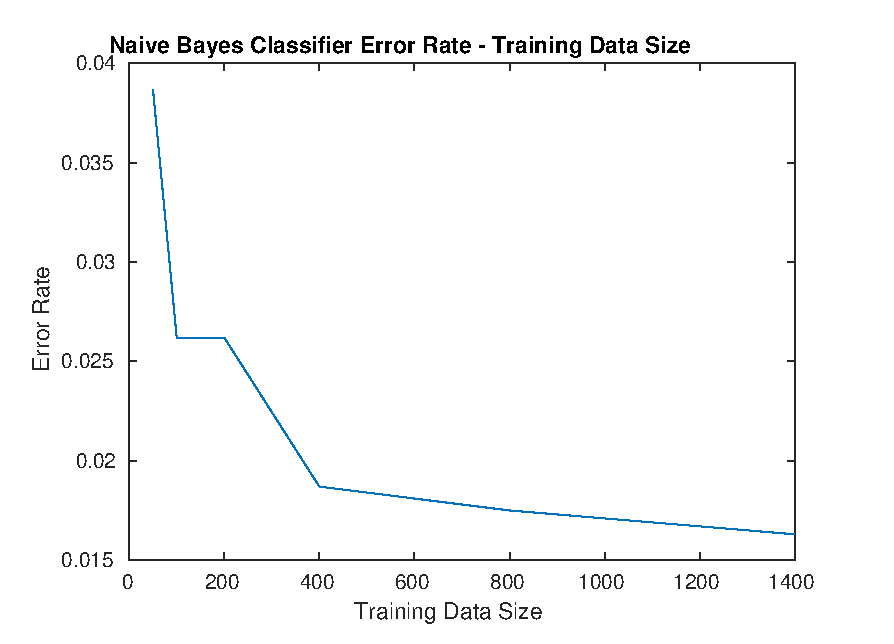
\includegraphics[scale = 1]{nb_error.eps}
	\caption{朴素贝叶斯分类器错误率-训练集大小}
\end{figure}

\subsection{}

考虑使用下面的技巧向量化核函数的计算,注意

\begin{equation}
	||x-z||_2^2 = \sum_i (x_i - z_i)^2 = \sum_i x_i^2 + z_i^2 - 2x_i z_i = \sum_i x_i^2 + \sum_i z_i^2 - 2 x^T z
\end{equation}

写出如下训练代码

\begin{lstlisting}[language = MATLAB]
alphas = zeros(40, numTrainDocs);

tau = 8;
TrainMatrix = full(Xtrain);
WordVectorLengthSquare = sum(TrainMatrix .^ 2, 2);
t = bsxfun(@plus, WordVectorLengthSquare, WordVectorLengthSquare');
K = exp(-(t - 2 .* TrainMatrix * TrainMatrix')/(2 * tau^2));

for j = 1:40
	iteration = 1;
	alpha = zeros(numTrainDocs, 1);
	for i = randperm(numTrainDocs)
		if (K(:,i)' * alpha * ytrain(i,1) < 1)
			alpha = alpha - (1/(sqrt(iteration))) * (-ytrain(i,1) * K(:,i) + (1/64) * alpha(i,1) * K(:,i));
		else
			alpha = alpha - (1/(sqrt(iteration))) * ((1/64) * alpha(i,1) * K(:,i));
		end
		iteration = iteration + 1;
	end
	alphas(j,:) = alpha;
end

average_alpha = (sum(alphas) ./ 40)';
\end{lstlisting}

测试代码类似

\begin{lstlisting}[language = MATLAB]
TestMatrix = full(Xtest);
TestWordVectorLengthSquare = sum(TestMatrix .^ 2, 2);

KTest = -2 .* (TestMatrix * TrainMatrix');
KTest = bsxfun(@plus, KTest, TestWordVectorLengthSquare);
Ktest = bsxfun(@plus, KTest, WordVectorLengthSquare');
Ktest = exp(-Ktest ./ (2 * tau^2));
predictions = 2 .* ((Ktest * average_alpha) > 0)  - 1;
\end{lstlisting}

使用不同大小的训练集, 计算测试集误差

\begin{table}[ht]
	\centering
	\begin{tabular}{|c|c|}
		\hline
		Training data size & test error rate \\
		\hline
		50 & $3\%$\\
		100 & $1.38\%$\\
		200 & $0.50\%$\\
		400 & $0.25\%$\\
		800 & $0.13\%$\\
		1400 & $0\%$\\
		\hline
	\end{tabular}
	\caption{SVM分类器错误率-训练集大小关系}
\end{table}



\begin{figure}[ht]
	\centering
	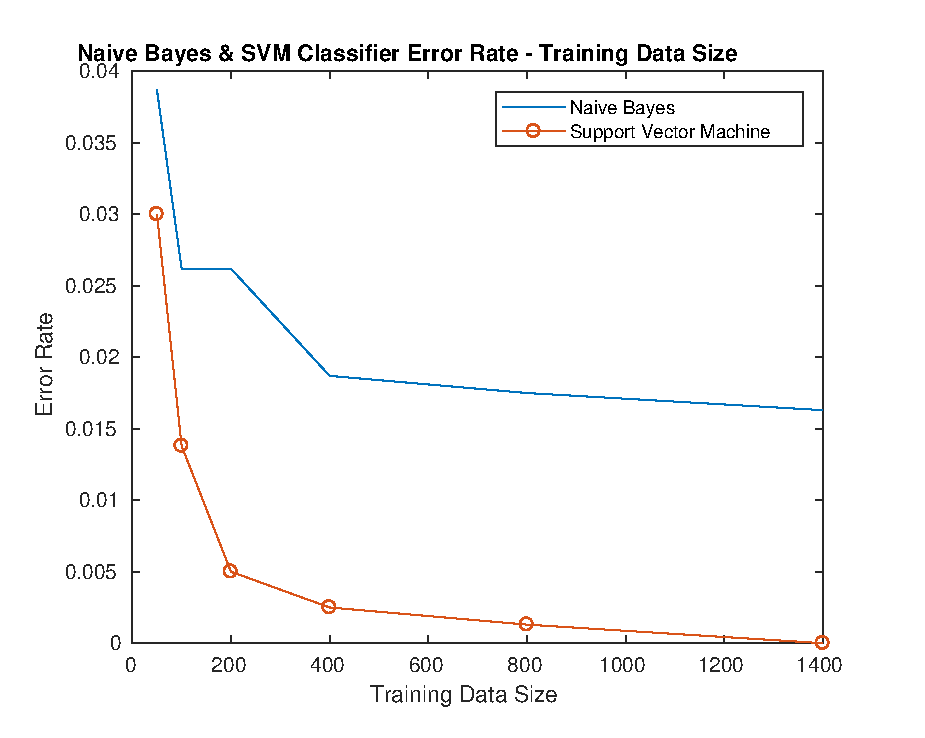
\includegraphics[scale = 1]{svm_error.eps}
	\caption{支持向量机分类器错误率-训练集大小}
\end{figure}

\subsection{}
朴素贝叶斯分类器和支持向量机分类器的错误率都随着训练集大小增大而减小, 但是支持向量机的错误率在任意训练集大小都低于朴素贝叶斯分类器, 同时, 支持向量机在样本量较小时性能并不稳定.

\section{Properties of VC Dimension}

\subsection{}

对于大小为$n$的某个点集, $n \le VC(H_1)$, 则存在$h \in H_1$, 能分割(shatter)该点集.由$H_1 \subseteq H_2$, $h \in H_2$, 故对于任意$n \le VC(H_1)$的点集, $H_2$中也至少有一个假设能够分割该点集, 那么根据定义有$VC(H_2) \ge VC(H_1)$.

\subsection{}
不妨取$k=1$.

对于$n = VC(H_1) + 1$的任意点集, 不存在$h \in H_1$分割该点集, 若对于$n = VC(H_1) + 1$的某个点集可被$h_1$分割, 则$H_1 \cup \{h_1\}$可分割$n \le VC(H_1) + 1$的点集, $VC(H_1) = VC(H_2) + 1$, 若任意$n = VC(H_1) + 1$的点集皆不可被$h_1$分割, $VC(H_1) = VC(H_2)$, 综上$VC(H_1) \le VC(H_2) + 1$.

对于$H_1 = H_2 \cup \{h_1, \cdots, h_k\}$

\begin{equation}
	VC(H_1) \le VC(H_2 \cup \{h_1, \cdots, h_{k-1}\}) + 1 \le VC(H_2 \cup \{h_1, \cdots, h_{k-2}\}) + 2 \le VC(H_1) + k
\end{equation}

\subsection{}



构造$h1:x = 0$, $h2:x=1$, $H1 = \{h1\}$, $H2 = \{ h2\}$.

注意到一条直线不能区分恰好落在主线上的单点集, 因此$VC(H_1) = VC(H_2) = 0$. 

而$VC(H_1 \cup H_2) = 1$, 因此该结论不成立.

\section{Training and testing on different distributions}
有
\begin{equation}
	\varepsilon_{\tau}(h) = (1 - \tau) \varepsilon_0(h) + \tau (1 - \varepsilon_0(h)) = (1 - 2\tau) \varepsilon_0(h) + \tau
\end{equation}

\begin{align*}
	\varepsilon_0(h) = \frac{(\varepsilon_\tau(h) - \tau)}{1-2\tau}
\end{align*}

\begin{align*}
	\varepsilon_0(\hat{h}) &= \frac{(\varepsilon_\tau(\hat{h}) - \tau)}{1-2\tau} \le \frac{(\hat{\varepsilon}_\tau(\hat{h}) + \gamma - \tau)}{1-2\tau} \le \frac{(\hat{\varepsilon}_\tau(h^*) + \gamma - \tau)}{1-2\tau} \\
	& \le \frac{({\varepsilon}_\tau(h^*) + 2\gamma - \tau)}{1-2\tau} = \varepsilon_0(h^*) + \frac{2\gamma}{1-2\tau}
\end{align*}

即

\begin{equation}
	\varepsilon_0(\hat{h}) \le \varepsilon_0(h^*) + \frac{2}{1-2\tau}\sqrt{\frac{1}{2m}\log(\frac{2|H|}{\delta})}
\end{equation}

给定$\delta, \gamma$, 保证$1- \delta$的置信度, 需要样本点
\begin{equation}
	m \ge \frac{1}{2(1-2\tau)^2\gamma^2}\log(\frac{2|H|}{\delta})
\end{equation}

当$\tau$接近$0.5$时, $\varepsilon_0(h)$迅速下降, 为保证误差和置信度所需的样本数量迅速上升, 最终趋近于无穷.

当标记误差足够大时, 训练集将完全失效.

\section{Boosting and High Energy Physics}

\subsection{}
对任意$s$, 总存在$k$满足

\begin{equation}
	x^{(1)} > x^{(2)} > \cdots x^{(k)} \ge s \ge x^{(k+1)} \cdots x^{(m-1)} > x^{(m)}
\end{equation}

取$m_0(s) = k$

\begin{align*}
	\sum_{i=1}^m p_i 1 \{\phi_{s,+}(x^{(i)}) \ne y^{(i)} \} &= \sum_{i=1}^{m_0(s)}\frac{(1 - y^{(i)})}{2}p_i + \sum_{m_0(s) + 1}^m\frac{(1 + y^{(i)})}{2}p_i \\
	&= \sum_{i=1}^m p_i - \frac{1}{2}(\sum_{i=1}^{m_0(s)} y^{(i)}p_i - \sum_{i = m_0(s) + 1}^m y^{(i)} p_i)
\end{align*}

类似的
\begin{align*}
\sum_{i=1}^m p_i 1 \{\phi_{s,+}(x^{(i)}) \ne y^{(i)} \} &= \sum_{i=1}^{m_0(s)}\frac{(1 + y^{(i)})}{2}p_i + \sum_{m_0(s) + 1}^m\frac{(1 - y^{(i)})}{2}p_i \\
&= \sum_{i=1}^m p_i + \frac{1}{2}(\sum_{i=1}^{m_0(s)} y^{(i)}p_i - \sum_{i = m_0(s) + 1}^m y^{(i)} p_i)
\end{align*}

\subsection{}

\begin{equation}
	f(m_0 + 1) - f(m_0) = 2y^{(m_0 + 1)}p_{m_0 + 1}
\end{equation}

得

\begin{equation}
	|f(m_0 + 1) - f(m_0)| = |2 y^{(m_0 + 1)} p_{m_0 + 1}| = 2p_{m_0 + 1}
\end{equation}

因此有

\begin{equation}
	\sum_{i=0}^{m-1} |f(i+1) - f(i)| = 2\sum_{i=0}^{m-1} p_{i+1} = 2
\end{equation}

因此存在$k$使得

\begin{equation*}
	|f(k+1) - f(k)| \ge \frac{2}{m}
\end{equation*}

因此必然有

\begin{equation*}
	|f(k+1)| \ge \frac{1}{m}  \text{  or  } |f(k)| \ge \frac{1}{m}
\end{equation*}

则$\gamma$可取为$\frac{1}{2m}$

\subsection{}

由于总存在$|f(m_0)| \ge 2 \gamma$, 总可以取到某一个阈值使得

\begin{equation}
	\sum_{i = 1}^{m} p_i 1{\phi(x^{(i)} \ne y^{(i)})} \le \frac{1}{2} - \gamma \notag
\end{equation}

$\gamma = \frac{1}{2m}$

由弱分类器上界

\begin{equation}
	t \ge \frac{\log(m)}{2 \gamma^2} = 2m^2 \log(m)
\end{equation}

\subsection{}

搜索最优特征和最优阈值的代码如下

\begin{lstlisting}[language = MATLAB]
err = zeros(1, nn);
threshs = zeros(1,nn);
for n = 1:nn
df = X(:,n);
[df_sort, df_ind] = sort(df, 'descend');
y_sort = y(df_ind);
p_sort = p_dist(df_ind);

yp = sum(y_sort .* p_sort);
p = 2 .* cumsum(y_sort .* p_sort) - yp;
p = 1/2 - p ./ 2;
[V, I] = max(abs(p - 0.5));
err(1, n) = min(p(I), 1 - p(I));
threshs(1, n) = df_sort(I);
end

[V, ind] = min(err);
thresh = threshs(1, ind);	
\end{lstlisting}

boost算法实现

\begin{lstlisting}[language = MATLAB]
w = ones(mm, 1);
for iter = 1:T
[ind, thresh] = find_best_threshold(X, y, p_dist);
feature_inds = [feature_inds; ind];
thresholds = [thresholds; thresh];
% ------- You should implement your code here -------- %
di = (((X(:,ind) > thresh) * 2) - 1) .* y;
W_plus = sum(w(di == 1));
W_minus = sum(w(di == -1));
newest_theta_param = (1/2) * log(W_plus/W_minus);  % Change this line so that newest_theta_param takes
% the optimal weight for the new decision stump.


% ------- No need to change this part ------- %
theta = [theta; newest_theta_param];
w = exp(-y .* (...
sign(X(:, feature_inds) - repmat(thresholds', mm, 1)) * theta));

p_dist = w / sum(w);	
\end{lstlisting}

random boost 算法实现

\begin{lstlisting}[language = MATLAB]
w = ones(mm, 1);
for iter = 1:T
ind = ceil(rand * nn);
thresh = X(ceil(rand * mm), ind) + 1e-8 * randn;

% ---- Your code here ----- %
di = (((X(:,ind) > thresh) * 2) - 1) .* y;
W_plus = sum(w(di == 1));
W_minus = sum(w(di == -1));
new_theta = (1/2) * log(W_plus/W_minus); % Modify this to use the optimal weight for the newest
% decision stump.

% ---- No need to touch this ---- %
theta = [theta; new_theta];
feature_inds = [feature_inds; ind];
thresholds = [thresholds; thresh];
w = exp(-y .* (sign(X(:, feature_inds) - repmat(thresholds', mm, 1)) * theta));
\end{lstlisting}

得到结果如图
\begin{figure}[ht]
	\parbox{0.5\textwidth}{	
		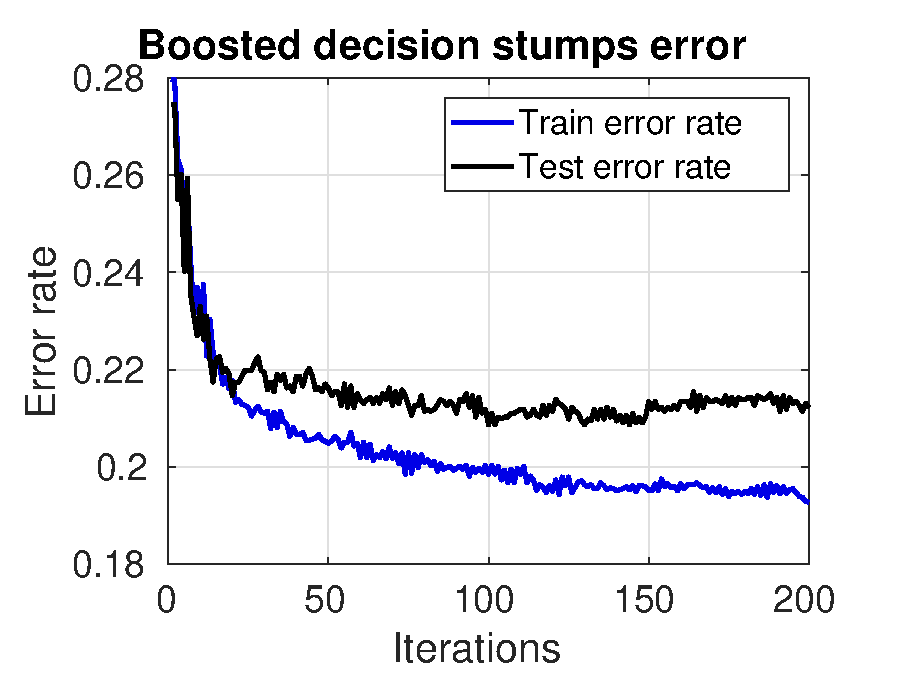
\includegraphics[width = 0.5\textwidth]{boost_nor.eps}
		\caption{boost decision stumps error}
	}
	\parbox{0.5\textwidth}{	
		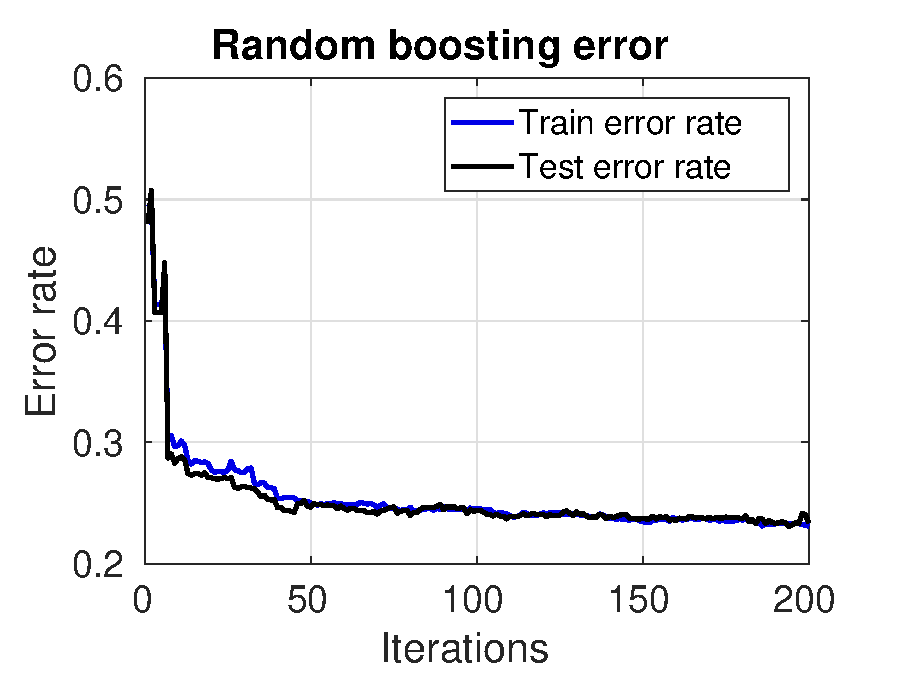
\includegraphics[width = 0.5\textwidth]{boost.eps}
		\caption{random boost error}
	}
\end{figure}

由图可知, boosted decision stumps 方法有一定的过拟合的趋势, 模型在测试集中工作的并不理想, 而random boosting方法则在训练集和测试集中都工作得比较好, 但正确率不如boosted decision stumps 方法.同时, boosted decision stumps 方法可以在更低的迭代次数下得到比较好的结果, 因此boosted decision stumps 方法更优.

\end{document}